\chapter*{Anonymisation des images DICOM}

Pour anonymiser les données, j'utilise le programme "Santé Dicom Editor". Il suffit d'ouvrir le dossier contenant les images et aller dans l'onglet Edit $\rightarrow$ Anonymise current file/series. Il existe des fonctions Matlab pour faire le même travail mais certains champs sensibles étaient malgré tous intacts. Voir \textit{http://www.santesoft.com/win/sante\_ dicom\_ editor/sante\_ dicom\_ editor.html}.

\begin{figure}[H]
\centering
    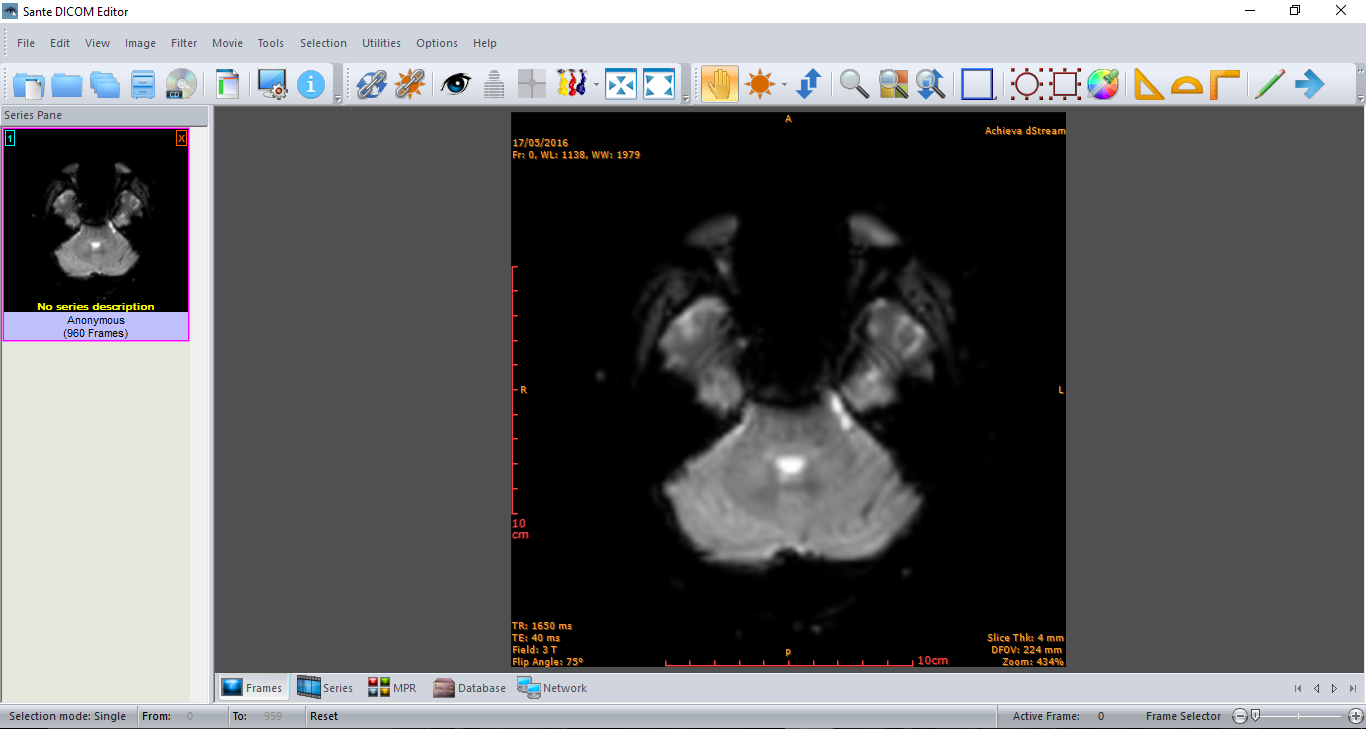
\includegraphics[scale=0.45,angle=90]{Images/AnonExe.png}
    \caption{Programme pour l'anonymisation des données.}
    \label{fig:AnonExe}
\end{figure}

\chapter*{Visualisation des données en 3D et 4D}

Un gros problème lorsque nous recevons les images Dicom est que nous ne pouvons voir de façon très claire la localisation de la tumeur. J'ai donc réutilisé et modifié des codes Matlab disponibles sur internet afin d'avoir une représentation 3D et 4D. Ils sont disponibles sur les liens suivant:

\medskip

\textit{http://fr.mathworks.com/matlabcentral/fileexchange/41465-4d-volume-visualization}

\textit{http://www.mathworks.com/matlabcentral/fileexchange/37268-3d-volume-visualization}

\medskip

Et sur le github du PFE :

\medskip

https://github.com/chuzelph-ENSTA-Bretagne/ThromboseIRM.git

\medskip

\begin{figure}[H]
\centering
    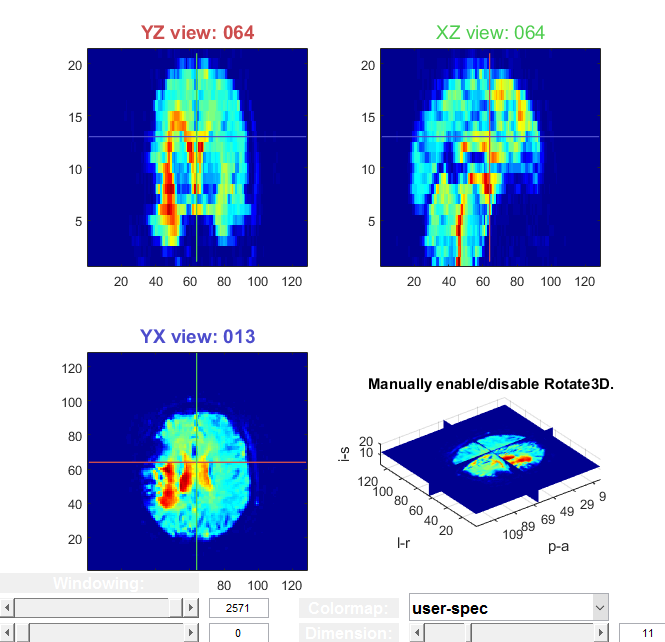
\includegraphics[scale=0.8,angle=0]{Images/4D.png}
    \caption{Programme Matlab pour la visualisation de données en 4D.}
    \label{fig:4D}
\end{figure}
